\chapter{Acoustics and Digital Signal Processing}
\label{ch:speech analysis}
In the past decade, digital computers have significantly helped \textit{signal processing} to quantify a finite number of bits. The flexibility inherited from digital elements allowed the usage of a vast number of techniques in which had been not possible to implement in the past. Nowadays, digital signal processor have been used to perform multiple operations, such as \textit{filtering}, \textit{spectrum estimation} and many others algorithms \cite{orfanidis1995introduction}.


\section{Speech signals}
\label{sec:speech_signals}
The \textbf{speech} is the human way of communication. The protocol used in communication is based on a syntactic combination of different words taken from a very large vocabulary. Each word in the vocabulary is composed by a small set of vowels and consonants that combined with a phonetic units form a spoken word. \\
\noindent When a word is pronounced\footnote{\ref{ch:english_language} explains in details how phonemes are pronunced}, a sounds is produced causing the air particles to be excited at a certain vibration rate. The source of our voice is due to the vibration of the vocal cords. The resultant signal is a \textit{non-stationary} but it can be divided in segments since each phoneme has a common acoustic properties. In \ref{fig:ex_sound_wave} is possible to notice how the pronounced words have a different shape as well as when the intensity of the voice is higher/lower during the pronunciation.
 
\begin{figure}[!ht]
	\centering
	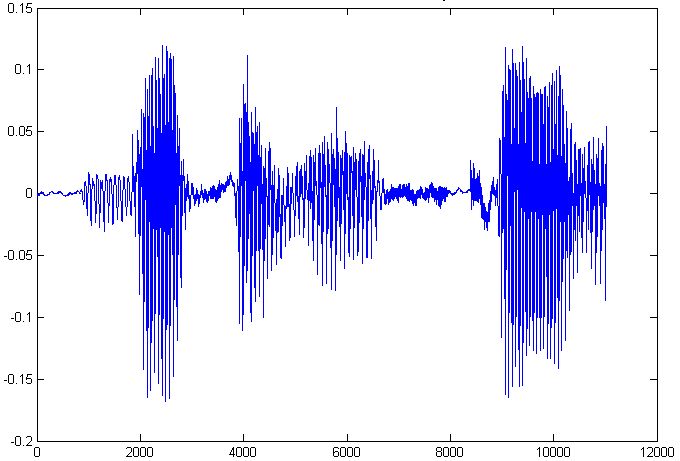
\includegraphics[scale=0.4]{Figures/ex_speech.png}
	\caption{Example of a speech sound. In this case, the sentence "This is a story" has been pronounced \cite{ex_speech_image}}
	\label{fig:ex_sound_wave}
\end{figure}

\noindent The simplest form of sound is the \textit{sinusoid} and it is the easiest waveform to describe because it corresponds to a \textbf{pure tone}. A pure tone consist in a waveform that consists only on one frequency. Other examples are the \textit{cosine} or \textit{sine} waves.

\subsection{Properties of Sinusoids}
\label{sub:prop_of_sinusoids}
A sinusoid, is a simple waveform represented by a up and down movement. There are three important measures that has to be taken into consideration when defining the shape of the sinusoid: \textit{amplitude}, \textit{frequency} and \textit{phase}. 

\subsubsection{Amplitude}
The amplitude, from a sound point of view, corresponds to the \textit{loudness} whereas in the soundwave it corresponds to the amount of \textbf{energy}. In general, to measure the amplitude, we use the unit called \textbf{deciBels} (dB) in which it is measured using a logarithmic scale relative to a standard sound \cite{prop_of_sinusoids}.

\subsubsection{Frequency}
Frequency is the number of cycles per unit of time\footnote{In general, a unit of time is considered a single second}.To define cycle, we can think of an oscillation that starts from the middle line, goes to the maximum point, down to the minimum and get back to the middle point. The unit of measure of the frequency is calculated in \textbf{Hertz} (Hz). Also, if we calculate the time taken for one cycle, we estimate the so called \textbf{period}. \\ 
\noindent Frequency plays a fundamental role with the \textit{pitch}. In fact, changing the number of oscillations but keeping the same waveform, we are able to increase or decrease the level of the pitch.

\subsubsection{Phase}
The \textbf{phase} measures the starting point position of the waveform. If the sinusoids start at the very minimum of the wave, the value of the phase is $\pi$ radians whereas starting from the top of the wave it will have a phase of \textit{zero}. When two sounds do not have the same phase, it is possible to perceive the difference in the time scale since one of the two is delayed compared to the other. When comparing two signals, there is the need to obtain a \textit{"phase-neutral"} that means the comparison is made taking only into account Amplitude and Frequency. This method is called \textbf{autocorrelation} of the signals.

\subsection{Spectrograms}
\label{sec:spectrograms}
A \textbf{Spectrogram} is the visual representation of an acoustic signal \cite{spectrogram_def}. Basically, a Fourier Transformation is applied to the sound, in such a way to obtain the set of waveforms extracted form the original signal and separate their frequencies and amplitudes. The result is typically depicted in a graph with degrees of amplitude with a \textit{light-dark} representation. Since amplitude represents the \textit{energy}, having a darker shade means that the energy is more intense in a certain range of frequencies - lighter when there is low energy. In \ref{fig:nasal_spectrogram} there is an example of the spectrogram. \\
\noindent The visual feedback of the spectrogram is highly dependent from the \textbf{window size} of the Fourier Analysis. In fact, different sizes affect the levels of frequencies and time resolution. \\
\noindent If the window size is \textit{short}, the adjacent \textbf{harmonics} are distorted but the time resolution is better \cite{spectrogram_def}. An harmonic is \textit{"an integer multiple of the fundamental frequency"}\cite{harmonic_wiki} or component frequencies. This is helpful when we are looking for the \textit{formant structure} because the striations created by the spectrogram highlights the individual pitch periods. \\
\noindent On the other hand, a \textit{wider} window size, helps to locate the harmonics because the band of the spectrogram are narrower.


\section{Fourier Analysis}
\label{sec:fourier_analysis}
\textbf{Fourier Analysis} is the process that decompose a periodic waveform into a set of sinusoids having different amplitudes, phases and frequencies. Yet, if we add those waveforms again, we will obtain the original signal. The analysis has been involved in many scientific applications and the reason is due to the following transform properties:

\begin{itemize}
	\item Linear transformation - the relationship between two modules is kept
	\item Exponential function are eigenfunctions of differentiation \cite{evans1997partial}
	\item Invertible - derived from the linear relationship
\end{itemize}

\noindent In signal processing, the Fourier analysis is used to isolate singular components of a complex waveform. A set of techniques consist in using \textbf{Fourier Transformation} on a signal in such a way to be able to manipulate the data in the easiest way possible but at the same time we have to be capable of inverting the transformation \cite{fa_wiki} \cite{rabiner1975theory}. In the next subsections we describe the fundamental steps for manipulating a signal.

\subsubsection{Sampling}
\label{ssubs:sampling}
\textit{Sampling} is the process that transform a continuous signal in to a discrete one. Each sample can be either be a single value or a set of values at a certain point in time \cite{sampling_wiki}. \\ 
\noindent Consider a sound signal that varies in time a continuous function $s(t)$. For every $T$ seconds, we need to measure the value of the function. This frame of time is called the \textit{sampling intervar} \cite{weik2012communications}. To calculate the sequence a sampled function is given as follow: $s(nT), \forall$ integer values of $n$. Thus, the \textit{sampling rate} is the average number of samples obtained in a range of $T = 1sec$ \cite{sampling_wiki}. An example of sampling is shown in \ref{fig:sampling_ex}.

\begin{figure}[!ht]
	\centering
	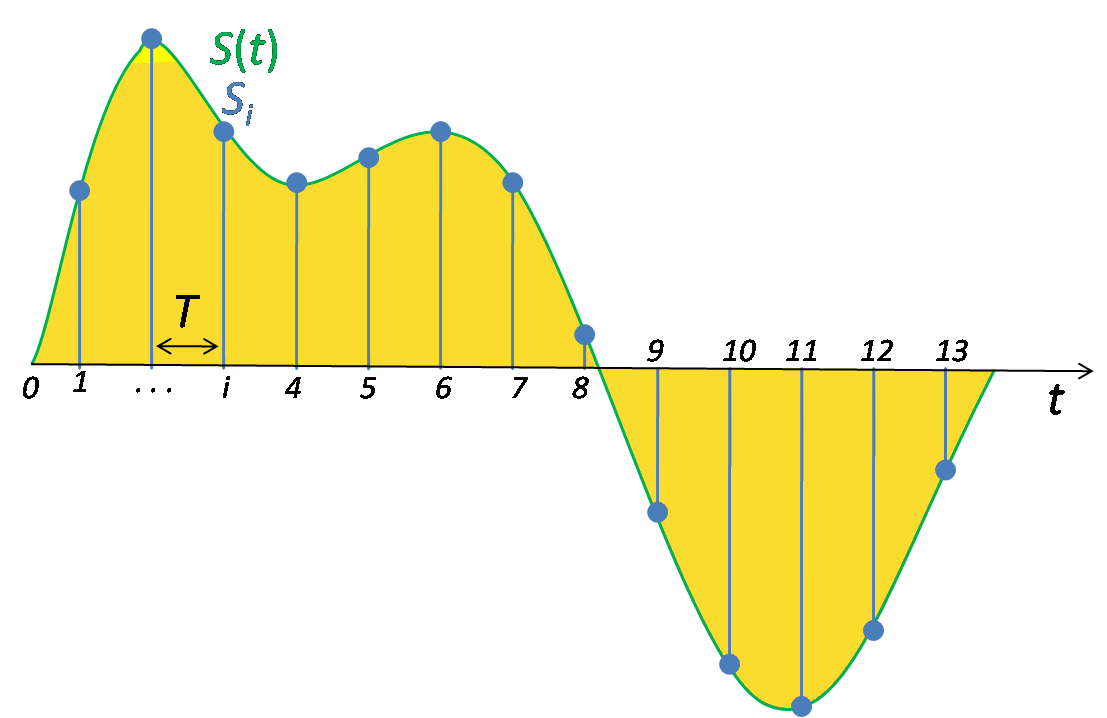
\includegraphics[scale=0.2]{Figures/sampling_example.png}
	\caption{Example of signal sampling. The green line represents the constinuous signal whereas the samples are represented by the blu lines \cite{sampling_wiki}}
	\label{fig:sampling_ex}
\end{figure}

\noindent As we mentioned above, using the Fourier Analysis we need to be able to reconstruct the original signal from the transformed one. To be able to, the \textbf{Nyquist-Shannon} theorem states that the sampling rate has to be larger as twice as the maximum frequency of the signal, in order to rebuild the original signal \cite{sampling_illinois}.\\
\noindent The \textit{Nyquist sampling rate} is defined by the following equation:

\begin{equation}
f_{s} > f_{Nyquist} = 2f_{max}
\end{equation}


\subsubsection{Quantization}
\label{subs:quantization}
To finalize the transformation from a continuous signal to a discrete one, we need to \textit{quantized} the signal in such a way to obtain a finite set of values. Unlike sampling in which permits to reconstruct the original signal, quantization is an irreversible operation that introduce a loss of information. \\
\noindent Consider $x$ be the sampled signal and $x_{q}$ the quantized one where $x_{q}$ can be expressed as the signal $x$ plus the error $e_{q}$. From here we have:

\begin{equation}
x_{q} = x + e{q} \Leftrightarrow e_{q} = x - x_{q}
\end{equation}

Given the equation above, we can restrict the range of error to $-q/2 ... +q/2$ because we will not make a larger error than the half of the quantization step. From a mathematical point of view, the error-signal is a random signal with an uniform probability distribution between the range of $−q/2 and +q/2$, giving the following \cite{quantization_math
	}:

\begin{equation}
p(e) = \begin{Bmatrix}
			\frac{1}{q} & for \frac{-q}{2} \leq  e < \frac{q}{2}\\ 
			0 			& otherwise
		\end{Bmatrix}
\end{equation}

Given this reason, the quantization error also called quantization noise.

\subsubsection{Windowing Signals}
\label{ssubs:windowing_signals}


\subsubsection{Zero Crossing Rate}
\label{ssubs:Zero Crossing Rate}


\subsubsection{Autocorrelation}
\label{ssubs:autocorrelation}



\section{Frequency Domain Analysis}
\label{sec:freq_domain_analysis}


\subsection{The Discrete Fourier Transform}
\label{sub:discrete_fourier_transform}
